\chapter{Forecasting}
\label{cap:prev}

\section{The best predictor}
For squared error, the best predictor of $y_{T+h}$ given the past is the conditional expectation $\E(y_{T+h}\mid y_T,y_{T-1},\dots)$ (chapter~\ref{cap:ec}). In an AR(1) with mean $\mu$:
\[
\hat y_{T+h}=\mu+\phi^h(y_T-\mu),\qquad \Var(e_{T+h})=\sigma^2\,\frac{1-\phi^{2h}}{1-\phi^2}.
\]
\begin{intuicao}
The farther the horizon, the more the forecast approaches the long-run mean, and the more the uncertainty approaches the unconditional variance $\gamma_0=\sigma^2/(1-\phi^2)$. For large $h$, the model knows no more than the mean.
\end{intuicao}

\begin{center}
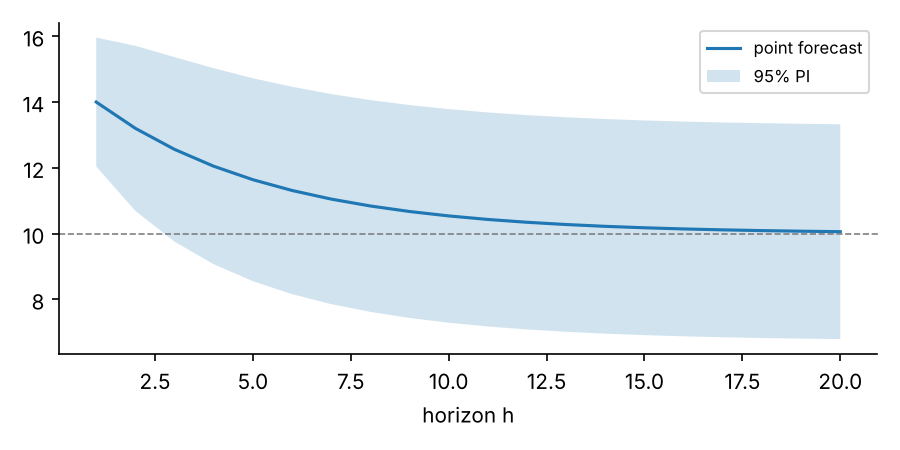
\includegraphics[width=0.75\textwidth]{fig/previsao_ar1.png}\\
\small AR(1) with $\mu=10$, $\phi=0.8$, $\sigma=1$ and last deviation $y_T-\mu=5$. The forecast decays to the mean and the interval widens and stabilizes.
\end{center}

\begin{simulacao}[Checked by simulation: interval coverage]
I simulated 4000 AR(1) series with $\phi=0.8$, forecast $h=3$ steps ahead and built the 95\% interval. The empirical coverage was $95.0\%$. The theoretical variance of the error for $h=3$ is $(1-0.8^6)/(1-0.64)=2.0496$, confirmed.
\end{simulacao}

\section{Random walk and ARIMA}
In a random walk, $\hat y_{T+h}=y_T$ (the ``naive'' forecast) and $\Var(e_{T+h})=h\sigma^2$. The interval grows without bound, which reflects the nature of permanent shocks. ARIMA models with $d\ge1$ have the same property, which is very different from a stationary model.

\begin{atencao}[Pitfall: optimistic intervals]
Classical intervals treat the estimated parameters as true and assume the model is right. With short samples or model choice made on the same data, the real coverage is usually lower than the nominal one. In serious forecasting, evaluate coverage out of sample.
\end{atencao}

\section{How to evaluate forecasts}
\begin{itemize}[leftmargin=1.4em]
\item \textbf{Out of sample, always.} In-sample fit rewards complicated models.
\item \textbf{Rolling origin}: estimate up to $t$, forecast $t+1,\dots,t+h$, move the origin forward and repeat.
\item \textbf{Metrics}: MAE and RMSE (same unit as the series); MAPE is intuitive, but explodes if there are values near zero and penalizes positive and negative errors asymmetrically; MASE compares with the naive forecaster and is comparable across series.
\item \textbf{Always include a benchmark}: naive (last value) or seasonal naive. A model that cannot beat the naive one is not worth using.
\end{itemize}

\begin{exercicio}
AR(1) with $\mu=0$, $\phi=0.8$, $\sigma^2=1$ and last value $y_T=5$. Give the forecast for $h=3$ and the 95\% interval.
\end{exercicio}
\sol{Forecast: $0.8^3\times5=0.512\times5=2.56$. Error variance: $2.0496$, standard deviation $1.4317$. Interval: $2.56\pm1.96\times1.4317=2.56\pm2.806$, that is, $[-0.25;\,5.37]$.}

\begin{exercicio}
A random walk has $\sigma=2$. What is the standard deviation of the 9-step-ahead forecast error?
\end{exercicio}
\sol{$\sqrt{h}\,\sigma=\sqrt9\times2=6$.}
